\documentclass[11pt,a4paper]{article}
\usepackage[utf8]{inputenc}
\usepackage[T1]{fontenc}
\usepackage{amsthm} %numéroter les questions
\usepackage[frenchb]{babel}
\usepackage{datetime}
\usepackage{xspace} % typographie IN
\usepackage{hyperref}% hyperliens
\usepackage[all]{hypcap} %lien pointe en haut des figures
\usepackage[french]{varioref} %voir x p y
\usepackage{fancyhdr}% en têtes
%\input cyracc.def
\usepackage[]{graphicx} %include pictures
\usepackage{pgfplots}
\usepackage[]{circuitikz}
\usepackage{ifthen}

\usepackage[top=1.3 in, bottom=1.3 in, left=1.3 in, right=1.3 in]{geometry} % Yeah, that's bad to play with margins
\usepackage[]{pdfpages}

\usepackage[]{attachfile}

\usepackage{float}
\usepackage{subfig}

\usepackage{todonotes} % \missingfigure
\usepackage{gensymb} % \ohm

\usepackage{framed}

\newdateformat{mydate}{2016--2017}%hack pour remplacer \THEYEAR


\newboolean{corrige}
\ifx\correction\undefined
\setboolean{corrige}{false}% pas de corrigé
\else
\setboolean{corrige}{true}%corrigé
\fi

%\setboolean{corrige}{false}% pas de corrigé

\newboolean{annexes}
\setboolean{annexes}{true}%annexes
%\setboolean{annexes}{false}% pas de annexes

\definecolor{darkblue}{rgb}{0,0,0.5}

\newboolean{mos}
%\setboolean{mos}{true}%annexes
\setboolean{mos}{false}% pas de annexes

\usepackage{aeguill} %guillemets

%% fancy header & foot
\pagestyle{fancy}
%Numero du TP :
\def \labonumber {Projet -- Partie 2}
\lhead{[ELEC-H-310] Choucroute numérique\\ \labonumber}
\rhead{\mydate\today\\ page \thepage}
\chead{\ifthenelse{\boolean{corrige}}{Corrigé}{}}
\cfoot{}
%%

\pdfinfo{
/Author (Quentin Delhaye, Ken Hasselmann, ULB -- BEAMS)
/Title (\labonumber ELEC-H-310)
/ModDate (D:\pdfdate)
}

\hypersetup{
pdftitle={\labonumber [ELEC-H-310] Choucroute numérique},
pdfauthor={Quentin Delhaye, Ken Hasselmann, ULB -- BEAMS},
pdfsubject={}
}

\theoremstyle{definition}% questions pas en italique
\newtheorem{Q}{Question}[] % numéroter les questions [section] ou non []

\newcommand{\reponse}[1]{% pour intégrer une réponse : \reponse{texte} : sera inclus si \boolean{corrige}
	\ifthenelse {\boolean{corrige}} {\paragraph{Réponse :} \color{darkblue}   #1\color{black}} {}
 }

\newcommand{\addcontentslinenono}[4]{\addtocontents{#1}{\protect\contentsline{#2}{#3}{#4}{}}}

\date{\vspace{-1.7cm}\mydate\today}
\title{\vspace{-2cm}\labonumber \\ Digital electronics [ELEC-H-310]\\Design of a cooling control system~: \\ acquisition and temperature control\ifthenelse{\boolean{corrige}}{~\\Corrigé}{}}

%\author{\vspace{-1cm}}%\textsc{Yannick Allard}}

\setlength{\parskip}{0.2cm plus2mm minus1mm} %espacement entre §
\setlength{\parindent}{0pt}


















\begin{document}
\pagestyle{empty}
\maketitle
% \vspace*{-1cm}




% ########   ##     ##  ##########  
% ##     ##  ##     ##      ##      
% ##     ##  ##     ##      ##      
% ########   ##     ##      ##      
% ##     ##  ##     ##      ##      
% ##     ##  ##     ##      ##      
% ########    #######       ##      

\section*{Aims}
During three laboratory sessions, you will have to design a small cooling control system based on a propeller fan.
You will also have to be able to interact locally (keyboard) with this system.

During the second lab session, you will implement a closed loop temperature control of an heating element.
You will have an effect on the temperature through the propeller fan.

\section*{Prerequisite}
Before entering in the lab, you have to read the project specifications defined in the file «~Design of a temperature regulation system~».


\section*{Objectives}
At the end of this lab session, you'll be able to~:
\begin{itemize}
	\item Size a data acquisition system for $\mu$C.
	\item Design and implement a simple control system.
\end{itemize}


\newpage




% ########   ##      ##  ##########  ########     #####    
%    ##      ###     ##      ##      ##     ##  ##     ##  
%    ##      ## ##   ##      ##      ##     ##  ##     ##  
%    ##      ##  ##  ##      ##      ########   ##     ##  
%    ##      ##   ## ##      ##      ##   ##    ##     ##  
%    ##      ##     ###      ##      ##    ##   ##     ##  
% ########   ##      ##      ##      ##     ##    #####    


\section{Introduction}
During three laboratory sessions, you will have to design a small cooling control system based on a propeller fan.
You will also have to be able to interact locally (keyboard) with this system.

During this second lab, your first aim will be to measure the temperature of a heating element.
In order to do this, you have to design a data acquisition system allowing to amplify a voltage representing the current temperature.

On the basis of this measure, and of the desired temperature, you will design a controller insuring the temperature of the element is the desired one.






%    ###      #######     #####    ##     ##  ########    #######   ########   ##########  ########     #####    ##      ##  
%   ## ##    ##     ##  ##     ##  ##     ##     ##      ##     ##     ##          ##         ##      ##     ##  ###     ##  
%  ##   ##   ##         ##     ##  ##     ##     ##      ##            ##          ##         ##      ##     ##  ## ##   ##  
% ##     ##  ##         ##     ##  ##     ##     ##       #######      ##          ##         ##      ##     ##  ##  ##  ##  
% #########  ##         ##    # #  ##     ##     ##             ##     ##          ##         ##      ##     ##  ##   ## ##  
% ##     ##  ##     ##    #### #   ##     ##     ##      ##     ##     ##          ##         ##      ##     ##  ##     ###  
% ##     ##   #######           #   #######   ########    #######   ########       ##      ########     #####    ##      ##  



\section{Design of the data acquisition system}
As explained in the project specifications, the measure of the temperature is realized by flowing a known continuous electrical current through a resistor whose the value change with temperature.

This measure, with a low amplitude, must then be amplified before being digitized (see figure~\ref{fig:acquisition}).

\begin{figure}[H]
\center
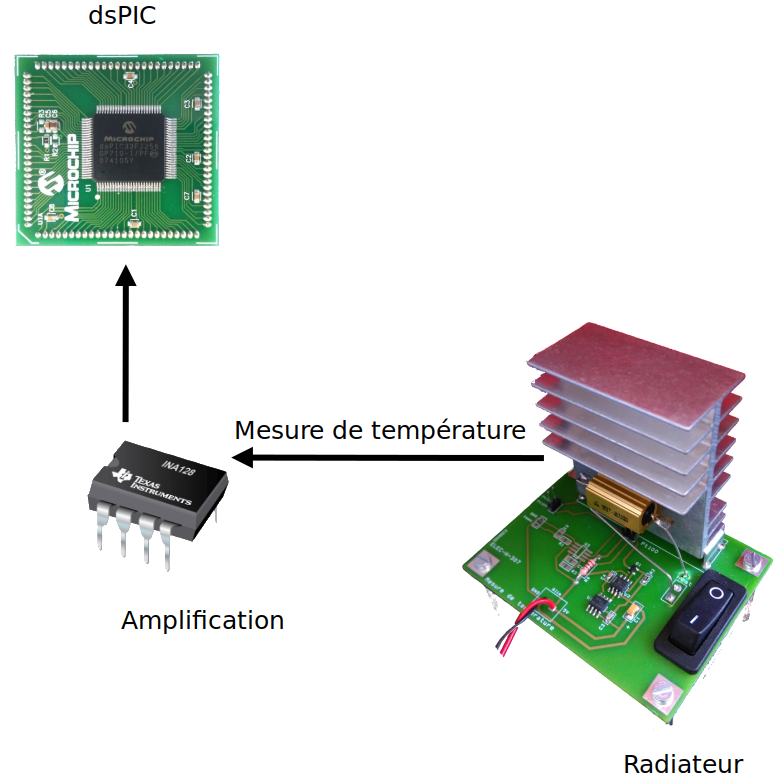
\includegraphics[width=0.8\textwidth]{acquisition}
\caption{Chaîne d'acquisition de la température.}
\label{fig:acquisition}
\end{figure}

\begin{itemize}
	\item Knowning that the temperature can reach 45$\celsius$, what is the maximum voltage measurable at the terminals of the resistor~?
	\item As the analog-to-digital converter digitizes the voltage on 10 bits and is supplied with 3.3V, what is its resolution~?
\end{itemize}

Now, we will design and implement the data acquisition system.
\begin{itemize}
	\item Why is it required to amplify~?
	\item Why this amplification must be differential~?
	\item Thanks to the datasheet of INA128, size the gain resistor.
	\item Realized the circuit on your protoboard and check if it works.
\end{itemize}






%  #######     #####    ##      ##  #########  ########    #######   ##     ##  ########      ###     ##########  ########     #####    ##      ##  
% ##     ##  ##     ##  ###     ##  ##            ##      ##         ##     ##  ##     ##    ## ##        ##         ##      ##     ##  ###     ##  
% ##         ##     ##  ## ##   ##  ##            ##      ##         ##     ##  ##     ##   ##   ##       ##         ##      ##     ##  ## ##   ##  
% ##         ##     ##  ##  ##  ##  ######        ##      ##   ####  ##     ##  ########   ##     ##      ##         ##      ##     ##  ##  ##  ##  
% ##         ##     ##  ##   ## ##  ##            ##      ##     ##  ##     ##  ##   ##    #########      ##         ##      ##     ##  ##   ## ##  
% ##     ##  ##     ##  ##     ###  ##            ##      ##     ##  ##     ##  ##    ##   ##     ##      ##         ##      ##     ##  ##     ###  
%  #######     #####    ##      ##  ##         ########   ########    #######   ##     ##  ##     ##      ##      ########     #####    ##      ##  



\section{Configuration of the analog-to-digital converter}
Now, you will program the analog-to-digital converter so that you obtain a "digital image" of the temperature.
\begin{itemize}
	\item Thanks to the coding guide (guide de programmation), configure the converter so that the temperature value is digitized each 10~ms (pay attention, additional steps are required in comparison with lab session 2).
	\item On the basis of your data acquisition system, write a function allowing to have the temperature in $\celsius$ from the number given at the output of the converter.
	\item Write a second function allowing to display the temperature on the LCD screen, with a refresh rate of one second.
\end{itemize}






% ########   #########   #######   ##     ##  ##            ###     ##########  ########     #####    ##      ##  
% ##     ##  ##         ##         ##     ##  ##           ## ##        ##         ##      ##     ##  ###     ##  
% ##     ##  ##         ##         ##     ##  ##          ##   ##       ##         ##      ##     ##  ## ##   ##  
% ########   ######     ##   ####  ##     ##  ##         ##     ##      ##         ##      ##     ##  ##  ##  ##  
% ##   ##    ##         ##     ##  ##     ##  ##         #########      ##         ##      ##     ##  ##   ## ##  
% ##    ##   ##         ##     ##  ##     ##  ##         ##     ##      ##         ##      ##     ##  ##     ###  
% ##     ##  #########  ########    #######   #########  ##     ##      ##      ########     #####    ##      ##  



\section{Temperature control}
You have now all the elements to realize our temperature control system.
The only thing missing is a controller (figure~\ref{fig:regulation}).

\begin{figure}[h]
\center
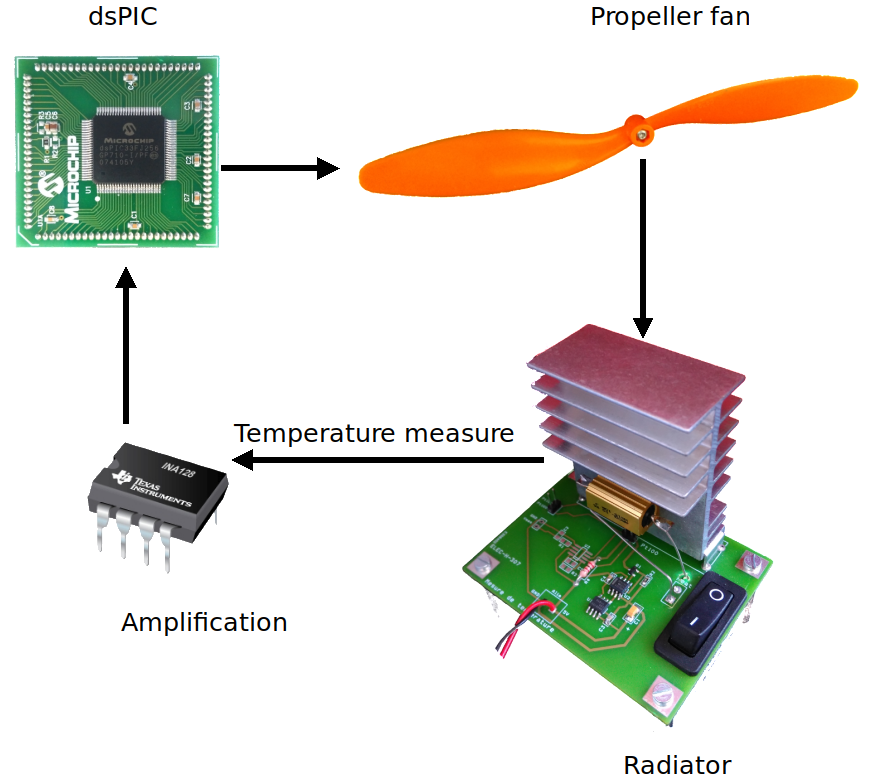
\includegraphics[width=0.8\textwidth]{regulation}
\caption{Boucle de régulation}
\label{fig:regulation}
\end{figure}

\begin{itemize}
	\item Write a function taking as an argument the desired temperature and the current temperature.
	This control function will have to adjust the rotation speed of the propeller fan, so that it regulates the temperature.
	The choice of the controller is up to you, but there no need to implement a too much complex one.
	\item Choose a reference (or desired) temperature of 28$\celsius$, and check if your system works.
\end{itemize}



\end{document}
